section*{Extra Credit 4: Discrete Diffusion (LLaDA) Ablation}

% \subsection*{Background: Discrete Diffusion for Text}
% Unlike continuous diffusion models (e.g., in image generation) that add Gaussian noise to a continuous state space, language relies on discrete tokens. Discrete diffusion adapts this framework by replacing Gaussian noise corruption with discrete state transitions—most commonly, replacing true tokens with a designated \texttt{[MASK]} token.

% Let $x_0 = [x_0^1, x_0^2, \dots, x_0^N]$ be the initial uncorrupted sequence of tokens from a vocabulary $V$. The forward process gradually corrupts $x_0$ over time $t \in [0, 1]$ into a noisy state $x_t$, where the final state $x_1$ is a sequence entirely composed of \texttt{[MASK]} tokens. The transition probability for a single token can be defined via a transition matrix $Q_t$:
% \begin{equation}
% q(x_t \mid x_{t-1}) = \text{Categorical}(x_t; x_{t-1} Q_t)
% \end{equation}
% where $Q_t$ absorbs tokens into the \texttt{[MASK]} state with increasing probability as $t \to 1$.

% The reverse process, parameterized by a neural network $p_\theta$ (in our case, LLaDA), learns to denoise the sequence. Instead of predicting $x_{t-1}$ directly, masking-based discrete diffusion models typically predict the fully clean sequence $p_\theta(\tilde{x}_0 \mid x_t)$. The intermediate state $x_{t-1}$ is then sampled using the posterior:
% \begin{equation}
% p_\theta(x_{t-1} \mid x_t) = \sum_{\tilde{x}_0} q(x_{t-1} \mid x_t, \tilde{x}_0) p_\theta(\tilde{x}_0 \mid x_t)
% \end{equation}
% At inference time, generation begins from a fully masked sequence $x_1$. The model iteratively predicts the clean sequence $\tilde{x}_0$, commits to the highest-confidence tokens, and re-masks the lowest-confidence tokens to produce $x_{t-1}$, stepping backwards until the final uncorrupted sequence $x_0$ is generated.

\subsection*{Methodology}
In this experiment, we evaluated the performance of LLaDA-8B on the Alien CalcGPT dataset. Unlike traditional autoregressive models that generate text sequentially from left to right, LLaDA utilizes the discrete diffusion process outlined above. This approach allows us to vary the number of sampling steps at inference time. We used a standard System Prompting strategy (providing definitions of the alien operators in the system message) and evaluated the model using $T \in \{8, 16, 32, 64\}$ diffusion steps to determine the optimal tradeoff between computational cost and mathematical reasoning accuracy. 

\subsection*{Unmasking Schedule}
In our implementation, the target sequence of length $N$ is initially filled entirely with mask tokens. Over $T$ diffusion steps, the model predicts and commits to a subset of tokens. The number of tokens unmasked at step $t$, denoted as $k_t$, follows a uniform linear schedule defined by:
\begin{equation}
k_t = 
\begin{cases} 
\lfloor \frac{N}{T} \rfloor + 1 & \text{if } t \le (N \bmod T) \\
\lfloor \frac{N}{T} \rfloor & \text{otherwise}
\end{cases}
\end{equation}
This ensures that the total number of mask tokens decreases evenly over time, forcing the model to iteratively refine its low-confidence predictions until all $N$ tokens are fully realized.

\subsection*{Quantitative Results}

The empirical results of the step ablation study are detailed in Table \ref{tab:llada_results}. 

\begin{table}[h]
\centering
\begin{tabular}{l c c c c c}
\toprule
\textbf{Diffusion Steps} & \textbf{Overall Acc.} & \textbf{Level 1 Acc.} & \textbf{Level 2 Acc.} & \textbf{Level 3 Acc.} & \textbf{Format Failures} \\
\midrule
$T = 8$  & 44.0\% (66/150)  & 36.0\%  & 82.0\%  & 14.0\%  & 29 \\
$T = 16$ & 52.7\% (79/150)  & 58.0\%  & 80.0\%  & 20.0\%  & 22 \\
$T = 32$ & \textbf{80.0\%} (120/150) & \textbf{100.0\%} & \textbf{98.0\%}  & \textbf{42.0\%}  & \textbf{0} \\
$T = 64$ & 78.0\% (117/150) & 100.0\% & 94.0\%  & 40.0\%  & 0 \\
\bottomrule
\end{tabular}
\caption{Accuracy of LLaDA-8B across different difficulty levels as a function of discrete diffusion steps.}
\label{tab:llada_results}
\end{table}

\begin{figure}[h]
    \centering
    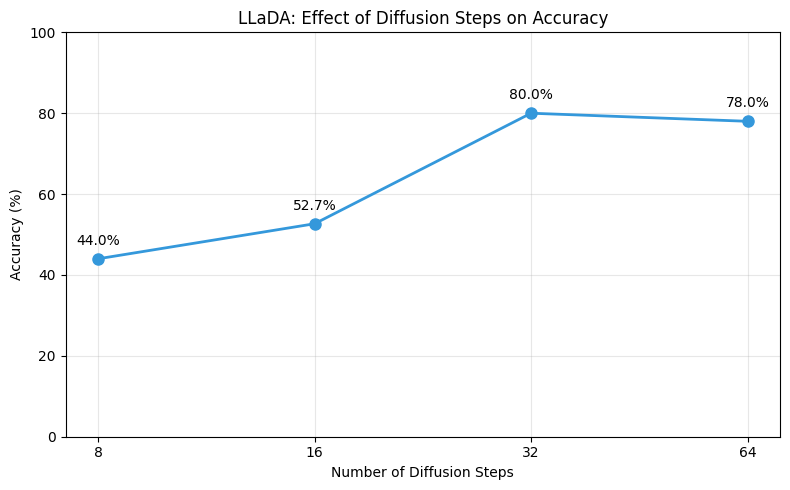
\includegraphics[width=0.48\textwidth]{llada_overall_acc_plot.png}
    \hfill
    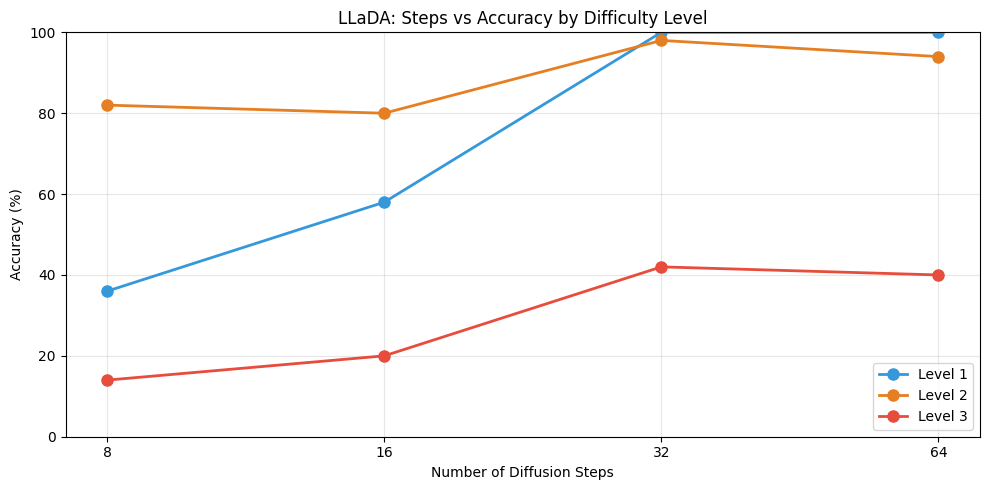
\includegraphics[width=0.48\textwidth]{llada_level_acc_plot.png}
    \caption{Left: Overall accuracy vs. number of diffusion steps. Right: Accuracy broken down by difficulty level across diffusion steps.}
    \label{fig:llada_plots}
\end{figure}

\subsection*{Analysis and Discussion}

The data reveals a stark performance threshold linked directly to the number of diffusion denoising steps:

\begin{itemize}
    \item \textbf{Low Step Counts ($T=8, 16$):} At lower step counts, the model struggles significantly, producing accuracies of 44.0\% and 52.7\%. A major symptom of this under-sampling is the high number of formatting failures (29 and 22, respectively). Applying Equation 3, when $T=8$ and our target sequence length is $N=64$, the model is forced to unmask exactly $k_t = 8$ tokens at every single step. Because it must commit to 8 tokens simultaneously without sufficient confidence, it fails to construct the required \texttt{Final Answer: <number>} syntax properly. Interestingly, at $T=8$, Level 1 accuracy (36.0\%) drops well below Level 2 accuracy (82.0\%). This artifact occurs because shorter target sequences (like Level 1 answers) suffer disproportionately from aggressive unmasking schedules; committing to 8 tokens per step for a very short answer effectively turns generation into a 1-shot or 2-shot blind guess, causing catastrophic logical errors early in the sequence.
    
    \item \textbf{Optimal Step Count ($T=32$):} Performance peaks at $T=32$, achieving an impressive \textbf{80.0\% overall accuracy}. With $k_t = 2$ tokens unmasked per step, the model has sufficient granular control to correct early mistakes before committing to them. As a result, format failures completely disappear. The model demonstrates perfect reasoning on Level 1 (100\%), near-perfect reasoning on Level 2 (98\%), and correctly solves 42\% of the highly complex, nested Level 3 problems.
    
    \item \textbf{Diminishing Returns ($T=64$):} Increasing the steps to $T=64$ yields no further benefit, causing a slight degradation to 78.0\% overall accuracy. This indicates that $T=32$ serves as the saturation point for reasoning capability on this specific context length, and computing further diffusion steps is unnecessary.
\end{itemize}

\subsection*{Qualitative Examples}

When the model is given sufficient steps ($T=64$), it can handle large arithmetic operations seamlessly:
\begin{itemize}
    \item \textbf{Success:} \texttt{glorp(trok(19, 18))} $\rightarrow$ Expected: 342 | Got: 342
    \item \textbf{Success:} \texttt{glorp(flarn(11, 16))} $\rightarrow$ Expected: 27 | Got: 27
\end{itemize}

However, when errors do occur on complex problems, they tend to represent failures in nested evaluation tracking rather than syntax errors:
\begin{itemize}
    \item \textbf{Failure:} \texttt{glorp(flarn(snib(12, 4), 4))} \\
    \textit{Standard Evaluation:} $(12 - 4) + 4 = 12$ \\
    \textit{Model Output:} \texttt{Final Answer: 8}
    \item \textbf{Failure:} \texttt{glorp(flarn(4, snib(19, 12)))} \\
    \textit{Standard Evaluation:} $4 + (19 - 12) = 11$ \\
    \textit{Model Output:} \texttt{Final Answer: 7}
\end{itemize}
In these Level 3 failures, the model performs the inner nested operation correctly (e.g., $12-4=8$, and $19-12=7$) but fails to propagate that intermediate result through the outer \texttt{flarn} (addition) operator, simply outputting the intermediate state as the final answer.
\end{itemize}